\documentclass[a4paper,10pt]{article}
\usepackage[margin=22mm]{geometry}
\usepackage{lipsum,amsmath,amsthm,tikz}
\usepackage[colorlinks=true,linkcolor=blue,urlcolor=blue]{hyperref}
\newtheorem{theorem}{Theorem}[section]
\newtheorem{lemma}[theorem]{Lemma}
\title{A varied document for sustained live editing}
\author{TeXpresso local profiling corpus}
\date{}
\begin{document}
\maketitle
The anchors EARLY, MIDDLE and LATE are unique source locations. Cross references
lead to Sections~\ref{unit:1}, \ref{unit:22} and \ref{unit:43},
and Equation~\ref{eq:1}. The accented words caf\'{e} and na\"ive coexist with
Unicode source comments; no external bibliography, image, or shell command is needed.
% Unicode offset sentinel: café 😀 章节

\section{A changing estimate: case 001}\label{unit:0}
A local change should remain attached to its source even when surrounding material moves. We compare the displayed argument with the current source version, rather than treating the last compiled page number as a permanent identity.

\lipsum[1-2]
\begin{align}\label{eq:0}
 F_k(x+h)&=F_k(x)+hF_k'(x)+\frac{h^2}{2}F_k''(x)+O(h^3),\\
 \int_0^1 t^k(1-t)\,dt&=\frac{1}{(k+1)(k+2)}.
\end{align}
\begin{lemma}\label{thm:0}
For the finite family in case 1, the normalized error is bounded by $C_k h^2$ whenever $0<h<1$. The constant may depend on $k$ but is independent of the location of the edited paragraph.
\end{lemma}
\begin{proof}
Expand the two terms, collect their first-order contributions, and apply the
triangle inequality. The remaining integral is bounded on the compact interval,
so the asserted estimate follows. This argument also applies after a line break
moves the statement to the next page.
\end{proof}
The next comparison uses Theorem~\ref{thm:0} and Equation~\ref{eq:0}. An observer can return to an earlier part of the document while compilation continues. The relevant statement, equation and hyperlink must still belong to the page actually displayed, including when line wrapping pushes a later theorem across a page boundary.

\lipsum[3]

\section{A changing estimate: case 002}\label{unit:1}
\hypertarget{varied:early}{}\label{anchor:early}
\noindent \texttt{EARLY-0001}: This uniquely marked paragraph remains visible as nearby text, mathematical statements and section boundaries change.
%<VARIED-CURSOR:early>

The construction uses a finite family of examples with different paragraph lengths. Some sentences are short. Others follow the dependence of an estimate on its parameters, introduce a counterexample, and explain why a nearby bound must be reconsidered after an insertion.

\lipsum[4-5]
\begin{align}\label{eq:1}
 F_k(x+h)&=F_k(x)+hF_k'(x)+\frac{h^2}{2}F_k''(x)+O(h^3),\\
 \int_0^1 t^k(1-t)\,dt&=\frac{1}{(k+1)(k+2)}.
\end{align}
\begin{theorem}\label{thm:1}
For the finite family in case 2, the normalized error is bounded by $C_k h^2$ whenever $0<h<1$. The constant may depend on $k$ but is independent of the location of the edited paragraph.
\end{theorem}
\begin{proof}
Expand the two terms, collect their first-order contributions, and apply the
triangle inequality. The remaining integral is bounded on the compact interval,
so the asserted estimate follows. This argument also applies after a line break
moves the statement to the next page.
\end{proof}
The next comparison uses Theorem~\ref{thm:0} and Equation~\ref{eq:1}. The proof separates the algebraic estimate from the geometric example. This makes the document useful for edits to prose, formulas, headings and diagrams, while retaining enough ordinary text to exercise paragraph breaking and natural pagination.

\lipsum[8]

\section{A changing estimate: case 003}\label{unit:2}
An observer can return to an earlier part of the document while compilation continues. The relevant statement, equation and hyperlink must still belong to the page actually displayed, including when line wrapping pushes a later theorem across a page boundary.

\lipsum[7-8]
\begin{align}\label{eq:2}
 F_k(x+h)&=F_k(x)+hF_k'(x)+\frac{h^2}{2}F_k''(x)+O(h^3),\\
 \int_0^1 t^k(1-t)\,dt&=\frac{1}{(k+1)(k+2)}.
\end{align}
\begin{theorem}\label{thm:2}
For the finite family in case 3, the normalized error is bounded by $C_k h^2$ whenever $0<h<1$. The constant may depend on $k$ but is independent of the location of the edited paragraph.
\end{theorem}
\begin{proof}
Expand the two terms, collect their first-order contributions, and apply the
triangle inequality. The remaining integral is bounded on the compact interval,
so the asserted estimate follows. This argument also applies after a line break
moves the statement to the next page.
\end{proof}
The next comparison uses Theorem~\ref{thm:1} and Equation~\ref{eq:2}. A local change should remain attached to its source even when surrounding material moves. We compare the displayed argument with the current source version, rather than treating the last compiled page number as a permanent identity.

\lipsum[13]

\section{A changing estimate: case 004}\label{unit:3}
The proof separates the algebraic estimate from the geometric example. This makes the document useful for edits to prose, formulas, headings and diagrams, while retaining enough ordinary text to exercise paragraph breaking and natural pagination.

\lipsum[10-11]
\begin{align}\label{eq:3}
 F_k(x+h)&=F_k(x)+hF_k'(x)+\frac{h^2}{2}F_k''(x)+O(h^3),\\
 \int_0^1 t^k(1-t)\,dt&=\frac{1}{(k+1)(k+2)}.
\end{align}
\begin{lemma}\label{thm:3}
For the finite family in case 4, the normalized error is bounded by $C_k h^2$ whenever $0<h<1$. The constant may depend on $k$ but is independent of the location of the edited paragraph.
\end{lemma}
\begin{proof}
Expand the two terms, collect their first-order contributions, and apply the
triangle inequality. The remaining integral is bounded on the compact interval,
so the asserted estimate follows. This argument also applies after a line break
moves the statement to the next page.
\end{proof}
\begin{center}
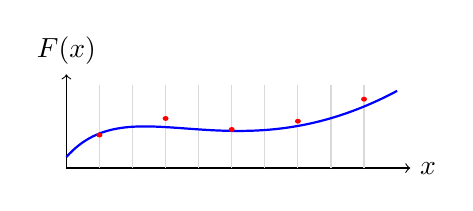
\begin{tikzpicture}[x=0.42cm,y=0.35cm]
 \draw[->] (0,0)--(10.4,0) node[right] {$x$};
 \draw[->] (0,0)--(0,3.4) node[above] {$F(x)$};
 \foreach \x in {1,...,9} {\draw[gray!30] (\x,0)--(\x,3);}
 \draw[blue,thick] (0,0.4) .. controls (2,3.1) and (5,-0.4) .. (10,2.8);
 \foreach \x/\y in {1/1.2,3/1.8,5/1.4,7/1.7,9/2.5}
   \fill[red] (\x,\y) circle (0.09);
\end{tikzpicture}
\end{center}
The next comparison uses Theorem~\ref{thm:2} and Equation~\ref{eq:3}. The construction uses a finite family of examples with different paragraph lengths. Some sentences are short. Others follow the dependence of an estimate on its parameters, introduce a counterexample, and explain why a nearby bound must be reconsidered after an insertion.

\lipsum[18]

\section{A changing estimate: case 005}\label{unit:4}
A local change should remain attached to its source even when surrounding material moves. We compare the displayed argument with the current source version, rather than treating the last compiled page number as a permanent identity.

\lipsum[13-14]
\begin{align}\label{eq:4}
 F_k(x+h)&=F_k(x)+hF_k'(x)+\frac{h^2}{2}F_k''(x)+O(h^3),\\
 \int_0^1 t^k(1-t)\,dt&=\frac{1}{(k+1)(k+2)}.
\end{align}
\begin{theorem}\label{thm:4}
For the finite family in case 5, the normalized error is bounded by $C_k h^2$ whenever $0<h<1$. The constant may depend on $k$ but is independent of the location of the edited paragraph.
\end{theorem}
\begin{proof}
Expand the two terms, collect their first-order contributions, and apply the
triangle inequality. The remaining integral is bounded on the compact interval,
so the asserted estimate follows. This argument also applies after a line break
moves the statement to the next page.
\end{proof}
The next comparison uses Theorem~\ref{thm:3} and Equation~\ref{eq:4}. An observer can return to an earlier part of the document while compilation continues. The relevant statement, equation and hyperlink must still belong to the page actually displayed, including when line wrapping pushes a later theorem across a page boundary.

\lipsum[23]

\section{A changing estimate: case 006}\label{unit:5}
The construction uses a finite family of examples with different paragraph lengths. Some sentences are short. Others follow the dependence of an estimate on its parameters, introduce a counterexample, and explain why a nearby bound must be reconsidered after an insertion.

\lipsum[16-17]
\begin{align}\label{eq:5}
 F_k(x+h)&=F_k(x)+hF_k'(x)+\frac{h^2}{2}F_k''(x)+O(h^3),\\
 \int_0^1 t^k(1-t)\,dt&=\frac{1}{(k+1)(k+2)}.
\end{align}
\begin{theorem}\label{thm:5}
For the finite family in case 6, the normalized error is bounded by $C_k h^2$ whenever $0<h<1$. The constant may depend on $k$ but is independent of the location of the edited paragraph.
\end{theorem}
\begin{proof}
Expand the two terms, collect their first-order contributions, and apply the
triangle inequality. The remaining integral is bounded on the compact interval,
so the asserted estimate follows. This argument also applies after a line break
moves the statement to the next page.
\end{proof}
The next comparison uses Theorem~\ref{thm:4} and Equation~\ref{eq:5}. The proof separates the algebraic estimate from the geometric example. This makes the document useful for edits to prose, formulas, headings and diagrams, while retaining enough ordinary text to exercise paragraph breaking and natural pagination.

\lipsum[3]

\section{A changing estimate: case 007}\label{unit:6}
An observer can return to an earlier part of the document while compilation continues. The relevant statement, equation and hyperlink must still belong to the page actually displayed, including when line wrapping pushes a later theorem across a page boundary.

\lipsum[19-20]
\begin{align}\label{eq:6}
 F_k(x+h)&=F_k(x)+hF_k'(x)+\frac{h^2}{2}F_k''(x)+O(h^3),\\
 \int_0^1 t^k(1-t)\,dt&=\frac{1}{(k+1)(k+2)}.
\end{align}
\begin{lemma}\label{thm:6}
For the finite family in case 7, the normalized error is bounded by $C_k h^2$ whenever $0<h<1$. The constant may depend on $k$ but is independent of the location of the edited paragraph.
\end{lemma}
\begin{proof}
Expand the two terms, collect their first-order contributions, and apply the
triangle inequality. The remaining integral is bounded on the compact interval,
so the asserted estimate follows. This argument also applies after a line break
moves the statement to the next page.
\end{proof}
The next comparison uses Theorem~\ref{thm:5} and Equation~\ref{eq:6}. A local change should remain attached to its source even when surrounding material moves. We compare the displayed argument with the current source version, rather than treating the last compiled page number as a permanent identity.

\lipsum[8]

\section{A changing estimate: case 008}\label{unit:7}
The proof separates the algebraic estimate from the geometric example. This makes the document useful for edits to prose, formulas, headings and diagrams, while retaining enough ordinary text to exercise paragraph breaking and natural pagination.

\lipsum[22-23]
\begin{align}\label{eq:7}
 F_k(x+h)&=F_k(x)+hF_k'(x)+\frac{h^2}{2}F_k''(x)+O(h^3),\\
 \int_0^1 t^k(1-t)\,dt&=\frac{1}{(k+1)(k+2)}.
\end{align}
\begin{theorem}\label{thm:7}
For the finite family in case 8, the normalized error is bounded by $C_k h^2$ whenever $0<h<1$. The constant may depend on $k$ but is independent of the location of the edited paragraph.
\end{theorem}
\begin{proof}
Expand the two terms, collect their first-order contributions, and apply the
triangle inequality. The remaining integral is bounded on the compact interval,
so the asserted estimate follows. This argument also applies after a line break
moves the statement to the next page.
\end{proof}
The next comparison uses Theorem~\ref{thm:6} and Equation~\ref{eq:7}. The construction uses a finite family of examples with different paragraph lengths. Some sentences are short. Others follow the dependence of an estimate on its parameters, introduce a counterexample, and explain why a nearby bound must be reconsidered after an insertion.

\lipsum[13]

\section{A changing estimate: case 009}\label{unit:8}
A local change should remain attached to its source even when surrounding material moves. We compare the displayed argument with the current source version, rather than treating the last compiled page number as a permanent identity.

\lipsum[25-26]
\begin{align}\label{eq:8}
 F_k(x+h)&=F_k(x)+hF_k'(x)+\frac{h^2}{2}F_k''(x)+O(h^3),\\
 \int_0^1 t^k(1-t)\,dt&=\frac{1}{(k+1)(k+2)}.
\end{align}
\begin{theorem}\label{thm:8}
For the finite family in case 9, the normalized error is bounded by $C_k h^2$ whenever $0<h<1$. The constant may depend on $k$ but is independent of the location of the edited paragraph.
\end{theorem}
\begin{proof}
Expand the two terms, collect their first-order contributions, and apply the
triangle inequality. The remaining integral is bounded on the compact interval,
so the asserted estimate follows. This argument also applies after a line break
moves the statement to the next page.
\end{proof}
The next comparison uses Theorem~\ref{thm:7} and Equation~\ref{eq:8}. An observer can return to an earlier part of the document while compilation continues. The relevant statement, equation and hyperlink must still belong to the page actually displayed, including when line wrapping pushes a later theorem across a page boundary.

\lipsum[18]

\section{A changing estimate: case 010}\label{unit:9}
The construction uses a finite family of examples with different paragraph lengths. Some sentences are short. Others follow the dependence of an estimate on its parameters, introduce a counterexample, and explain why a nearby bound must be reconsidered after an insertion.

\lipsum[28-29]
\begin{align}\label{eq:9}
 F_k(x+h)&=F_k(x)+hF_k'(x)+\frac{h^2}{2}F_k''(x)+O(h^3),\\
 \int_0^1 t^k(1-t)\,dt&=\frac{1}{(k+1)(k+2)}.
\end{align}
\begin{lemma}\label{thm:9}
For the finite family in case 10, the normalized error is bounded by $C_k h^2$ whenever $0<h<1$. The constant may depend on $k$ but is independent of the location of the edited paragraph.
\end{lemma}
\begin{proof}
Expand the two terms, collect their first-order contributions, and apply the
triangle inequality. The remaining integral is bounded on the compact interval,
so the asserted estimate follows. This argument also applies after a line break
moves the statement to the next page.
\end{proof}
\begin{center}
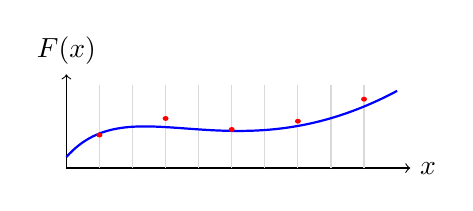
\begin{tikzpicture}[x=0.42cm,y=0.35cm]
 \draw[->] (0,0)--(10.4,0) node[right] {$x$};
 \draw[->] (0,0)--(0,3.4) node[above] {$F(x)$};
 \foreach \x in {1,...,9} {\draw[gray!30] (\x,0)--(\x,3);}
 \draw[blue,thick] (0,0.4) .. controls (2,3.1) and (5,-0.4) .. (10,2.8);
 \foreach \x/\y in {1/1.2,3/1.8,5/1.4,7/1.7,9/2.5}
   \fill[red] (\x,\y) circle (0.09);
\end{tikzpicture}
\end{center}
The next comparison uses Theorem~\ref{thm:8} and Equation~\ref{eq:9}. The proof separates the algebraic estimate from the geometric example. This makes the document useful for edits to prose, formulas, headings and diagrams, while retaining enough ordinary text to exercise paragraph breaking and natural pagination.

\lipsum[23]

\section{A changing estimate: case 011}\label{unit:10}
An observer can return to an earlier part of the document while compilation continues. The relevant statement, equation and hyperlink must still belong to the page actually displayed, including when line wrapping pushes a later theorem across a page boundary.

\lipsum[1-2]
\begin{align}\label{eq:10}
 F_k(x+h)&=F_k(x)+hF_k'(x)+\frac{h^2}{2}F_k''(x)+O(h^3),\\
 \int_0^1 t^k(1-t)\,dt&=\frac{1}{(k+1)(k+2)}.
\end{align}
\begin{theorem}\label{thm:10}
For the finite family in case 11, the normalized error is bounded by $C_k h^2$ whenever $0<h<1$. The constant may depend on $k$ but is independent of the location of the edited paragraph.
\end{theorem}
\begin{proof}
Expand the two terms, collect their first-order contributions, and apply the
triangle inequality. The remaining integral is bounded on the compact interval,
so the asserted estimate follows. This argument also applies after a line break
moves the statement to the next page.
\end{proof}
The next comparison uses Theorem~\ref{thm:9} and Equation~\ref{eq:10}. A local change should remain attached to its source even when surrounding material moves. We compare the displayed argument with the current source version, rather than treating the last compiled page number as a permanent identity.

\lipsum[3]

\section{A changing estimate: case 012}\label{unit:11}
The proof separates the algebraic estimate from the geometric example. This makes the document useful for edits to prose, formulas, headings and diagrams, while retaining enough ordinary text to exercise paragraph breaking and natural pagination.

\lipsum[4-5]
\begin{align}\label{eq:11}
 F_k(x+h)&=F_k(x)+hF_k'(x)+\frac{h^2}{2}F_k''(x)+O(h^3),\\
 \int_0^1 t^k(1-t)\,dt&=\frac{1}{(k+1)(k+2)}.
\end{align}
\begin{theorem}\label{thm:11}
For the finite family in case 12, the normalized error is bounded by $C_k h^2$ whenever $0<h<1$. The constant may depend on $k$ but is independent of the location of the edited paragraph.
\end{theorem}
\begin{proof}
Expand the two terms, collect their first-order contributions, and apply the
triangle inequality. The remaining integral is bounded on the compact interval,
so the asserted estimate follows. This argument also applies after a line break
moves the statement to the next page.
\end{proof}
The next comparison uses Theorem~\ref{thm:10} and Equation~\ref{eq:11}. The construction uses a finite family of examples with different paragraph lengths. Some sentences are short. Others follow the dependence of an estimate on its parameters, introduce a counterexample, and explain why a nearby bound must be reconsidered after an insertion.

\lipsum[8]

\section{A changing estimate: case 013}\label{unit:12}
A local change should remain attached to its source even when surrounding material moves. We compare the displayed argument with the current source version, rather than treating the last compiled page number as a permanent identity.

\lipsum[7-8]
\begin{align}\label{eq:12}
 F_k(x+h)&=F_k(x)+hF_k'(x)+\frac{h^2}{2}F_k''(x)+O(h^3),\\
 \int_0^1 t^k(1-t)\,dt&=\frac{1}{(k+1)(k+2)}.
\end{align}
\begin{lemma}\label{thm:12}
For the finite family in case 13, the normalized error is bounded by $C_k h^2$ whenever $0<h<1$. The constant may depend on $k$ but is independent of the location of the edited paragraph.
\end{lemma}
\begin{proof}
Expand the two terms, collect their first-order contributions, and apply the
triangle inequality. The remaining integral is bounded on the compact interval,
so the asserted estimate follows. This argument also applies after a line break
moves the statement to the next page.
\end{proof}
The next comparison uses Theorem~\ref{thm:11} and Equation~\ref{eq:12}. An observer can return to an earlier part of the document while compilation continues. The relevant statement, equation and hyperlink must still belong to the page actually displayed, including when line wrapping pushes a later theorem across a page boundary.

\lipsum[13]

\section{A changing estimate: case 014}\label{unit:13}
The construction uses a finite family of examples with different paragraph lengths. Some sentences are short. Others follow the dependence of an estimate on its parameters, introduce a counterexample, and explain why a nearby bound must be reconsidered after an insertion.

\lipsum[10-11]
\begin{align}\label{eq:13}
 F_k(x+h)&=F_k(x)+hF_k'(x)+\frac{h^2}{2}F_k''(x)+O(h^3),\\
 \int_0^1 t^k(1-t)\,dt&=\frac{1}{(k+1)(k+2)}.
\end{align}
\begin{theorem}\label{thm:13}
For the finite family in case 14, the normalized error is bounded by $C_k h^2$ whenever $0<h<1$. The constant may depend on $k$ but is independent of the location of the edited paragraph.
\end{theorem}
\begin{proof}
Expand the two terms, collect their first-order contributions, and apply the
triangle inequality. The remaining integral is bounded on the compact interval,
so the asserted estimate follows. This argument also applies after a line break
moves the statement to the next page.
\end{proof}
The next comparison uses Theorem~\ref{thm:12} and Equation~\ref{eq:13}. The proof separates the algebraic estimate from the geometric example. This makes the document useful for edits to prose, formulas, headings and diagrams, while retaining enough ordinary text to exercise paragraph breaking and natural pagination.

\lipsum[18]

\section{A changing estimate: case 015}\label{unit:14}
An observer can return to an earlier part of the document while compilation continues. The relevant statement, equation and hyperlink must still belong to the page actually displayed, including when line wrapping pushes a later theorem across a page boundary.

\lipsum[13-14]
\begin{align}\label{eq:14}
 F_k(x+h)&=F_k(x)+hF_k'(x)+\frac{h^2}{2}F_k''(x)+O(h^3),\\
 \int_0^1 t^k(1-t)\,dt&=\frac{1}{(k+1)(k+2)}.
\end{align}
\begin{theorem}\label{thm:14}
For the finite family in case 15, the normalized error is bounded by $C_k h^2$ whenever $0<h<1$. The constant may depend on $k$ but is independent of the location of the edited paragraph.
\end{theorem}
\begin{proof}
Expand the two terms, collect their first-order contributions, and apply the
triangle inequality. The remaining integral is bounded on the compact interval,
so the asserted estimate follows. This argument also applies after a line break
moves the statement to the next page.
\end{proof}
The next comparison uses Theorem~\ref{thm:13} and Equation~\ref{eq:14}. A local change should remain attached to its source even when surrounding material moves. We compare the displayed argument with the current source version, rather than treating the last compiled page number as a permanent identity.

\lipsum[23]

\section{A changing estimate: case 016}\label{unit:15}
The proof separates the algebraic estimate from the geometric example. This makes the document useful for edits to prose, formulas, headings and diagrams, while retaining enough ordinary text to exercise paragraph breaking and natural pagination.

\lipsum[16-17]
\begin{align}\label{eq:15}
 F_k(x+h)&=F_k(x)+hF_k'(x)+\frac{h^2}{2}F_k''(x)+O(h^3),\\
 \int_0^1 t^k(1-t)\,dt&=\frac{1}{(k+1)(k+2)}.
\end{align}
\begin{lemma}\label{thm:15}
For the finite family in case 16, the normalized error is bounded by $C_k h^2$ whenever $0<h<1$. The constant may depend on $k$ but is independent of the location of the edited paragraph.
\end{lemma}
\begin{proof}
Expand the two terms, collect their first-order contributions, and apply the
triangle inequality. The remaining integral is bounded on the compact interval,
so the asserted estimate follows. This argument also applies after a line break
moves the statement to the next page.
\end{proof}
\begin{center}
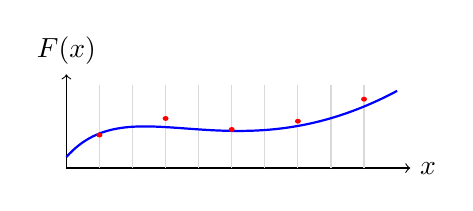
\begin{tikzpicture}[x=0.42cm,y=0.35cm]
 \draw[->] (0,0)--(10.4,0) node[right] {$x$};
 \draw[->] (0,0)--(0,3.4) node[above] {$F(x)$};
 \foreach \x in {1,...,9} {\draw[gray!30] (\x,0)--(\x,3);}
 \draw[blue,thick] (0,0.4) .. controls (2,3.1) and (5,-0.4) .. (10,2.8);
 \foreach \x/\y in {1/1.2,3/1.8,5/1.4,7/1.7,9/2.5}
   \fill[red] (\x,\y) circle (0.09);
\end{tikzpicture}
\end{center}
The next comparison uses Theorem~\ref{thm:14} and Equation~\ref{eq:15}. The construction uses a finite family of examples with different paragraph lengths. Some sentences are short. Others follow the dependence of an estimate on its parameters, introduce a counterexample, and explain why a nearby bound must be reconsidered after an insertion.

\lipsum[3]

\section{A changing estimate: case 017}\label{unit:16}
A local change should remain attached to its source even when surrounding material moves. We compare the displayed argument with the current source version, rather than treating the last compiled page number as a permanent identity.

\lipsum[19-20]
\begin{align}\label{eq:16}
 F_k(x+h)&=F_k(x)+hF_k'(x)+\frac{h^2}{2}F_k''(x)+O(h^3),\\
 \int_0^1 t^k(1-t)\,dt&=\frac{1}{(k+1)(k+2)}.
\end{align}
\begin{theorem}\label{thm:16}
For the finite family in case 17, the normalized error is bounded by $C_k h^2$ whenever $0<h<1$. The constant may depend on $k$ but is independent of the location of the edited paragraph.
\end{theorem}
\begin{proof}
Expand the two terms, collect their first-order contributions, and apply the
triangle inequality. The remaining integral is bounded on the compact interval,
so the asserted estimate follows. This argument also applies after a line break
moves the statement to the next page.
\end{proof}
The next comparison uses Theorem~\ref{thm:15} and Equation~\ref{eq:16}. An observer can return to an earlier part of the document while compilation continues. The relevant statement, equation and hyperlink must still belong to the page actually displayed, including when line wrapping pushes a later theorem across a page boundary.

\lipsum[8]

\section{A changing estimate: case 018}\label{unit:17}
The construction uses a finite family of examples with different paragraph lengths. Some sentences are short. Others follow the dependence of an estimate on its parameters, introduce a counterexample, and explain why a nearby bound must be reconsidered after an insertion.

\lipsum[22-23]
\begin{align}\label{eq:17}
 F_k(x+h)&=F_k(x)+hF_k'(x)+\frac{h^2}{2}F_k''(x)+O(h^3),\\
 \int_0^1 t^k(1-t)\,dt&=\frac{1}{(k+1)(k+2)}.
\end{align}
\begin{theorem}\label{thm:17}
For the finite family in case 18, the normalized error is bounded by $C_k h^2$ whenever $0<h<1$. The constant may depend on $k$ but is independent of the location of the edited paragraph.
\end{theorem}
\begin{proof}
Expand the two terms, collect their first-order contributions, and apply the
triangle inequality. The remaining integral is bounded on the compact interval,
so the asserted estimate follows. This argument also applies after a line break
moves the statement to the next page.
\end{proof}
The next comparison uses Theorem~\ref{thm:16} and Equation~\ref{eq:17}. The proof separates the algebraic estimate from the geometric example. This makes the document useful for edits to prose, formulas, headings and diagrams, while retaining enough ordinary text to exercise paragraph breaking and natural pagination.

\lipsum[13]

\section{A changing estimate: case 019}\label{unit:18}
An observer can return to an earlier part of the document while compilation continues. The relevant statement, equation and hyperlink must still belong to the page actually displayed, including when line wrapping pushes a later theorem across a page boundary.

\lipsum[25-26]
\begin{align}\label{eq:18}
 F_k(x+h)&=F_k(x)+hF_k'(x)+\frac{h^2}{2}F_k''(x)+O(h^3),\\
 \int_0^1 t^k(1-t)\,dt&=\frac{1}{(k+1)(k+2)}.
\end{align}
\begin{lemma}\label{thm:18}
For the finite family in case 19, the normalized error is bounded by $C_k h^2$ whenever $0<h<1$. The constant may depend on $k$ but is independent of the location of the edited paragraph.
\end{lemma}
\begin{proof}
Expand the two terms, collect their first-order contributions, and apply the
triangle inequality. The remaining integral is bounded on the compact interval,
so the asserted estimate follows. This argument also applies after a line break
moves the statement to the next page.
\end{proof}
The next comparison uses Theorem~\ref{thm:17} and Equation~\ref{eq:18}. A local change should remain attached to its source even when surrounding material moves. We compare the displayed argument with the current source version, rather than treating the last compiled page number as a permanent identity.

\lipsum[18]

\section{A changing estimate: case 020}\label{unit:19}
The proof separates the algebraic estimate from the geometric example. This makes the document useful for edits to prose, formulas, headings and diagrams, while retaining enough ordinary text to exercise paragraph breaking and natural pagination.

\lipsum[28-29]
\begin{align}\label{eq:19}
 F_k(x+h)&=F_k(x)+hF_k'(x)+\frac{h^2}{2}F_k''(x)+O(h^3),\\
 \int_0^1 t^k(1-t)\,dt&=\frac{1}{(k+1)(k+2)}.
\end{align}
\begin{theorem}\label{thm:19}
For the finite family in case 20, the normalized error is bounded by $C_k h^2$ whenever $0<h<1$. The constant may depend on $k$ but is independent of the location of the edited paragraph.
\end{theorem}
\begin{proof}
Expand the two terms, collect their first-order contributions, and apply the
triangle inequality. The remaining integral is bounded on the compact interval,
so the asserted estimate follows. This argument also applies after a line break
moves the statement to the next page.
\end{proof}
The next comparison uses Theorem~\ref{thm:18} and Equation~\ref{eq:19}. The construction uses a finite family of examples with different paragraph lengths. Some sentences are short. Others follow the dependence of an estimate on its parameters, introduce a counterexample, and explain why a nearby bound must be reconsidered after an insertion.

\lipsum[23]

\section{A changing estimate: case 021}\label{unit:20}
A local change should remain attached to its source even when surrounding material moves. We compare the displayed argument with the current source version, rather than treating the last compiled page number as a permanent identity.

\lipsum[1-2]
\begin{align}\label{eq:20}
 F_k(x+h)&=F_k(x)+hF_k'(x)+\frac{h^2}{2}F_k''(x)+O(h^3),\\
 \int_0^1 t^k(1-t)\,dt&=\frac{1}{(k+1)(k+2)}.
\end{align}
\begin{theorem}\label{thm:20}
For the finite family in case 21, the normalized error is bounded by $C_k h^2$ whenever $0<h<1$. The constant may depend on $k$ but is independent of the location of the edited paragraph.
\end{theorem}
\begin{proof}
Expand the two terms, collect their first-order contributions, and apply the
triangle inequality. The remaining integral is bounded on the compact interval,
so the asserted estimate follows. This argument also applies after a line break
moves the statement to the next page.
\end{proof}
The next comparison uses Theorem~\ref{thm:19} and Equation~\ref{eq:20}. An observer can return to an earlier part of the document while compilation continues. The relevant statement, equation and hyperlink must still belong to the page actually displayed, including when line wrapping pushes a later theorem across a page boundary.

\lipsum[3]

\section{A changing estimate: case 022}\label{unit:21}
The construction uses a finite family of examples with different paragraph lengths. Some sentences are short. Others follow the dependence of an estimate on its parameters, introduce a counterexample, and explain why a nearby bound must be reconsidered after an insertion.

\lipsum[4-5]
\begin{align}\label{eq:21}
 F_k(x+h)&=F_k(x)+hF_k'(x)+\frac{h^2}{2}F_k''(x)+O(h^3),\\
 \int_0^1 t^k(1-t)\,dt&=\frac{1}{(k+1)(k+2)}.
\end{align}
\begin{lemma}\label{thm:21}
For the finite family in case 22, the normalized error is bounded by $C_k h^2$ whenever $0<h<1$. The constant may depend on $k$ but is independent of the location of the edited paragraph.
\end{lemma}
\begin{proof}
Expand the two terms, collect their first-order contributions, and apply the
triangle inequality. The remaining integral is bounded on the compact interval,
so the asserted estimate follows. This argument also applies after a line break
moves the statement to the next page.
\end{proof}
\begin{center}
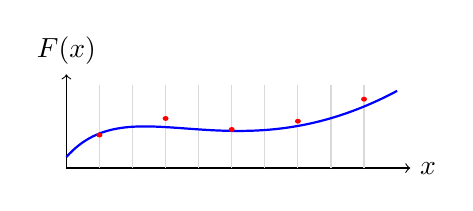
\begin{tikzpicture}[x=0.42cm,y=0.35cm]
 \draw[->] (0,0)--(10.4,0) node[right] {$x$};
 \draw[->] (0,0)--(0,3.4) node[above] {$F(x)$};
 \foreach \x in {1,...,9} {\draw[gray!30] (\x,0)--(\x,3);}
 \draw[blue,thick] (0,0.4) .. controls (2,3.1) and (5,-0.4) .. (10,2.8);
 \foreach \x/\y in {1/1.2,3/1.8,5/1.4,7/1.7,9/2.5}
   \fill[red] (\x,\y) circle (0.09);
\end{tikzpicture}
\end{center}
The next comparison uses Theorem~\ref{thm:20} and Equation~\ref{eq:21}. The proof separates the algebraic estimate from the geometric example. This makes the document useful for edits to prose, formulas, headings and diagrams, while retaining enough ordinary text to exercise paragraph breaking and natural pagination.

\lipsum[8]

\section{A changing estimate: case 023}\label{unit:22}
\hypertarget{varied:middle}{}\label{anchor:middle}
\noindent \texttt{MIDDLE-0022}: This uniquely marked paragraph remains visible as nearby text, mathematical statements and section boundaries change.
%<VARIED-CURSOR:middle>

An observer can return to an earlier part of the document while compilation continues. The relevant statement, equation and hyperlink must still belong to the page actually displayed, including when line wrapping pushes a later theorem across a page boundary.

\lipsum[7-8]
\begin{align}\label{eq:22}
 F_k(x+h)&=F_k(x)+hF_k'(x)+\frac{h^2}{2}F_k''(x)+O(h^3),\\
 \int_0^1 t^k(1-t)\,dt&=\frac{1}{(k+1)(k+2)}.
\end{align}
\begin{theorem}\label{thm:22}
For the finite family in case 23, the normalized error is bounded by $C_k h^2$ whenever $0<h<1$. The constant may depend on $k$ but is independent of the location of the edited paragraph.
\end{theorem}
\begin{proof}
Expand the two terms, collect their first-order contributions, and apply the
triangle inequality. The remaining integral is bounded on the compact interval,
so the asserted estimate follows. This argument also applies after a line break
moves the statement to the next page.
\end{proof}
The next comparison uses Theorem~\ref{thm:21} and Equation~\ref{eq:22}. A local change should remain attached to its source even when surrounding material moves. We compare the displayed argument with the current source version, rather than treating the last compiled page number as a permanent identity.

\lipsum[13]

\section{A changing estimate: case 024}\label{unit:23}
The proof separates the algebraic estimate from the geometric example. This makes the document useful for edits to prose, formulas, headings and diagrams, while retaining enough ordinary text to exercise paragraph breaking and natural pagination.

\lipsum[10-11]
\begin{align}\label{eq:23}
 F_k(x+h)&=F_k(x)+hF_k'(x)+\frac{h^2}{2}F_k''(x)+O(h^3),\\
 \int_0^1 t^k(1-t)\,dt&=\frac{1}{(k+1)(k+2)}.
\end{align}
\begin{theorem}\label{thm:23}
For the finite family in case 24, the normalized error is bounded by $C_k h^2$ whenever $0<h<1$. The constant may depend on $k$ but is independent of the location of the edited paragraph.
\end{theorem}
\begin{proof}
Expand the two terms, collect their first-order contributions, and apply the
triangle inequality. The remaining integral is bounded on the compact interval,
so the asserted estimate follows. This argument also applies after a line break
moves the statement to the next page.
\end{proof}
The next comparison uses Theorem~\ref{thm:22} and Equation~\ref{eq:23}. The construction uses a finite family of examples with different paragraph lengths. Some sentences are short. Others follow the dependence of an estimate on its parameters, introduce a counterexample, and explain why a nearby bound must be reconsidered after an insertion.

\lipsum[18]

\section{A changing estimate: case 025}\label{unit:24}
A local change should remain attached to its source even when surrounding material moves. We compare the displayed argument with the current source version, rather than treating the last compiled page number as a permanent identity.

\lipsum[13-14]
\begin{align}\label{eq:24}
 F_k(x+h)&=F_k(x)+hF_k'(x)+\frac{h^2}{2}F_k''(x)+O(h^3),\\
 \int_0^1 t^k(1-t)\,dt&=\frac{1}{(k+1)(k+2)}.
\end{align}
\begin{lemma}\label{thm:24}
For the finite family in case 25, the normalized error is bounded by $C_k h^2$ whenever $0<h<1$. The constant may depend on $k$ but is independent of the location of the edited paragraph.
\end{lemma}
\begin{proof}
Expand the two terms, collect their first-order contributions, and apply the
triangle inequality. The remaining integral is bounded on the compact interval,
so the asserted estimate follows. This argument also applies after a line break
moves the statement to the next page.
\end{proof}
The next comparison uses Theorem~\ref{thm:23} and Equation~\ref{eq:24}. An observer can return to an earlier part of the document while compilation continues. The relevant statement, equation and hyperlink must still belong to the page actually displayed, including when line wrapping pushes a later theorem across a page boundary.

\lipsum[23]

\section{A changing estimate: case 026}\label{unit:25}
The construction uses a finite family of examples with different paragraph lengths. Some sentences are short. Others follow the dependence of an estimate on its parameters, introduce a counterexample, and explain why a nearby bound must be reconsidered after an insertion.

\lipsum[16-17]
\begin{align}\label{eq:25}
 F_k(x+h)&=F_k(x)+hF_k'(x)+\frac{h^2}{2}F_k''(x)+O(h^3),\\
 \int_0^1 t^k(1-t)\,dt&=\frac{1}{(k+1)(k+2)}.
\end{align}
\begin{theorem}\label{thm:25}
For the finite family in case 26, the normalized error is bounded by $C_k h^2$ whenever $0<h<1$. The constant may depend on $k$ but is independent of the location of the edited paragraph.
\end{theorem}
\begin{proof}
Expand the two terms, collect their first-order contributions, and apply the
triangle inequality. The remaining integral is bounded on the compact interval,
so the asserted estimate follows. This argument also applies after a line break
moves the statement to the next page.
\end{proof}
The next comparison uses Theorem~\ref{thm:24} and Equation~\ref{eq:25}. The proof separates the algebraic estimate from the geometric example. This makes the document useful for edits to prose, formulas, headings and diagrams, while retaining enough ordinary text to exercise paragraph breaking and natural pagination.

\lipsum[3]

\section{A changing estimate: case 027}\label{unit:26}
An observer can return to an earlier part of the document while compilation continues. The relevant statement, equation and hyperlink must still belong to the page actually displayed, including when line wrapping pushes a later theorem across a page boundary.

\lipsum[19-20]
\begin{align}\label{eq:26}
 F_k(x+h)&=F_k(x)+hF_k'(x)+\frac{h^2}{2}F_k''(x)+O(h^3),\\
 \int_0^1 t^k(1-t)\,dt&=\frac{1}{(k+1)(k+2)}.
\end{align}
\begin{theorem}\label{thm:26}
For the finite family in case 27, the normalized error is bounded by $C_k h^2$ whenever $0<h<1$. The constant may depend on $k$ but is independent of the location of the edited paragraph.
\end{theorem}
\begin{proof}
Expand the two terms, collect their first-order contributions, and apply the
triangle inequality. The remaining integral is bounded on the compact interval,
so the asserted estimate follows. This argument also applies after a line break
moves the statement to the next page.
\end{proof}
The next comparison uses Theorem~\ref{thm:25} and Equation~\ref{eq:26}. A local change should remain attached to its source even when surrounding material moves. We compare the displayed argument with the current source version, rather than treating the last compiled page number as a permanent identity.

\lipsum[8]

\section{A changing estimate: case 028}\label{unit:27}
The proof separates the algebraic estimate from the geometric example. This makes the document useful for edits to prose, formulas, headings and diagrams, while retaining enough ordinary text to exercise paragraph breaking and natural pagination.

\lipsum[22-23]
\begin{align}\label{eq:27}
 F_k(x+h)&=F_k(x)+hF_k'(x)+\frac{h^2}{2}F_k''(x)+O(h^3),\\
 \int_0^1 t^k(1-t)\,dt&=\frac{1}{(k+1)(k+2)}.
\end{align}
\begin{lemma}\label{thm:27}
For the finite family in case 28, the normalized error is bounded by $C_k h^2$ whenever $0<h<1$. The constant may depend on $k$ but is independent of the location of the edited paragraph.
\end{lemma}
\begin{proof}
Expand the two terms, collect their first-order contributions, and apply the
triangle inequality. The remaining integral is bounded on the compact interval,
so the asserted estimate follows. This argument also applies after a line break
moves the statement to the next page.
\end{proof}
\begin{center}
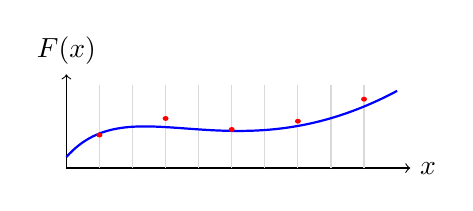
\begin{tikzpicture}[x=0.42cm,y=0.35cm]
 \draw[->] (0,0)--(10.4,0) node[right] {$x$};
 \draw[->] (0,0)--(0,3.4) node[above] {$F(x)$};
 \foreach \x in {1,...,9} {\draw[gray!30] (\x,0)--(\x,3);}
 \draw[blue,thick] (0,0.4) .. controls (2,3.1) and (5,-0.4) .. (10,2.8);
 \foreach \x/\y in {1/1.2,3/1.8,5/1.4,7/1.7,9/2.5}
   \fill[red] (\x,\y) circle (0.09);
\end{tikzpicture}
\end{center}
The next comparison uses Theorem~\ref{thm:26} and Equation~\ref{eq:27}. The construction uses a finite family of examples with different paragraph lengths. Some sentences are short. Others follow the dependence of an estimate on its parameters, introduce a counterexample, and explain why a nearby bound must be reconsidered after an insertion.

\lipsum[13]

\section{A changing estimate: case 029}\label{unit:28}
A local change should remain attached to its source even when surrounding material moves. We compare the displayed argument with the current source version, rather than treating the last compiled page number as a permanent identity.

\lipsum[25-26]
\begin{align}\label{eq:28}
 F_k(x+h)&=F_k(x)+hF_k'(x)+\frac{h^2}{2}F_k''(x)+O(h^3),\\
 \int_0^1 t^k(1-t)\,dt&=\frac{1}{(k+1)(k+2)}.
\end{align}
\begin{theorem}\label{thm:28}
For the finite family in case 29, the normalized error is bounded by $C_k h^2$ whenever $0<h<1$. The constant may depend on $k$ but is independent of the location of the edited paragraph.
\end{theorem}
\begin{proof}
Expand the two terms, collect their first-order contributions, and apply the
triangle inequality. The remaining integral is bounded on the compact interval,
so the asserted estimate follows. This argument also applies after a line break
moves the statement to the next page.
\end{proof}
The next comparison uses Theorem~\ref{thm:27} and Equation~\ref{eq:28}. An observer can return to an earlier part of the document while compilation continues. The relevant statement, equation and hyperlink must still belong to the page actually displayed, including when line wrapping pushes a later theorem across a page boundary.

\lipsum[18]

\section{A changing estimate: case 030}\label{unit:29}
The construction uses a finite family of examples with different paragraph lengths. Some sentences are short. Others follow the dependence of an estimate on its parameters, introduce a counterexample, and explain why a nearby bound must be reconsidered after an insertion.

\lipsum[28-29]
\begin{align}\label{eq:29}
 F_k(x+h)&=F_k(x)+hF_k'(x)+\frac{h^2}{2}F_k''(x)+O(h^3),\\
 \int_0^1 t^k(1-t)\,dt&=\frac{1}{(k+1)(k+2)}.
\end{align}
\begin{theorem}\label{thm:29}
For the finite family in case 30, the normalized error is bounded by $C_k h^2$ whenever $0<h<1$. The constant may depend on $k$ but is independent of the location of the edited paragraph.
\end{theorem}
\begin{proof}
Expand the two terms, collect their first-order contributions, and apply the
triangle inequality. The remaining integral is bounded on the compact interval,
so the asserted estimate follows. This argument also applies after a line break
moves the statement to the next page.
\end{proof}
The next comparison uses Theorem~\ref{thm:28} and Equation~\ref{eq:29}. The proof separates the algebraic estimate from the geometric example. This makes the document useful for edits to prose, formulas, headings and diagrams, while retaining enough ordinary text to exercise paragraph breaking and natural pagination.

\lipsum[23]

\section{A changing estimate: case 031}\label{unit:30}
An observer can return to an earlier part of the document while compilation continues. The relevant statement, equation and hyperlink must still belong to the page actually displayed, including when line wrapping pushes a later theorem across a page boundary.

\lipsum[1-2]
\begin{align}\label{eq:30}
 F_k(x+h)&=F_k(x)+hF_k'(x)+\frac{h^2}{2}F_k''(x)+O(h^3),\\
 \int_0^1 t^k(1-t)\,dt&=\frac{1}{(k+1)(k+2)}.
\end{align}
\begin{lemma}\label{thm:30}
For the finite family in case 31, the normalized error is bounded by $C_k h^2$ whenever $0<h<1$. The constant may depend on $k$ but is independent of the location of the edited paragraph.
\end{lemma}
\begin{proof}
Expand the two terms, collect their first-order contributions, and apply the
triangle inequality. The remaining integral is bounded on the compact interval,
so the asserted estimate follows. This argument also applies after a line break
moves the statement to the next page.
\end{proof}
The next comparison uses Theorem~\ref{thm:29} and Equation~\ref{eq:30}. A local change should remain attached to its source even when surrounding material moves. We compare the displayed argument with the current source version, rather than treating the last compiled page number as a permanent identity.

\lipsum[3]

\section{A changing estimate: case 032}\label{unit:31}
The proof separates the algebraic estimate from the geometric example. This makes the document useful for edits to prose, formulas, headings and diagrams, while retaining enough ordinary text to exercise paragraph breaking and natural pagination.

\lipsum[4-5]
\begin{align}\label{eq:31}
 F_k(x+h)&=F_k(x)+hF_k'(x)+\frac{h^2}{2}F_k''(x)+O(h^3),\\
 \int_0^1 t^k(1-t)\,dt&=\frac{1}{(k+1)(k+2)}.
\end{align}
\begin{theorem}\label{thm:31}
For the finite family in case 32, the normalized error is bounded by $C_k h^2$ whenever $0<h<1$. The constant may depend on $k$ but is independent of the location of the edited paragraph.
\end{theorem}
\begin{proof}
Expand the two terms, collect their first-order contributions, and apply the
triangle inequality. The remaining integral is bounded on the compact interval,
so the asserted estimate follows. This argument also applies after a line break
moves the statement to the next page.
\end{proof}
The next comparison uses Theorem~\ref{thm:30} and Equation~\ref{eq:31}. The construction uses a finite family of examples with different paragraph lengths. Some sentences are short. Others follow the dependence of an estimate on its parameters, introduce a counterexample, and explain why a nearby bound must be reconsidered after an insertion.

\lipsum[8]

\section{A changing estimate: case 033}\label{unit:32}
A local change should remain attached to its source even when surrounding material moves. We compare the displayed argument with the current source version, rather than treating the last compiled page number as a permanent identity.

\lipsum[7-8]
\begin{align}\label{eq:32}
 F_k(x+h)&=F_k(x)+hF_k'(x)+\frac{h^2}{2}F_k''(x)+O(h^3),\\
 \int_0^1 t^k(1-t)\,dt&=\frac{1}{(k+1)(k+2)}.
\end{align}
\begin{theorem}\label{thm:32}
For the finite family in case 33, the normalized error is bounded by $C_k h^2$ whenever $0<h<1$. The constant may depend on $k$ but is independent of the location of the edited paragraph.
\end{theorem}
\begin{proof}
Expand the two terms, collect their first-order contributions, and apply the
triangle inequality. The remaining integral is bounded on the compact interval,
so the asserted estimate follows. This argument also applies after a line break
moves the statement to the next page.
\end{proof}
The next comparison uses Theorem~\ref{thm:31} and Equation~\ref{eq:32}. An observer can return to an earlier part of the document while compilation continues. The relevant statement, equation and hyperlink must still belong to the page actually displayed, including when line wrapping pushes a later theorem across a page boundary.

\lipsum[13]

\section{A changing estimate: case 034}\label{unit:33}
The construction uses a finite family of examples with different paragraph lengths. Some sentences are short. Others follow the dependence of an estimate on its parameters, introduce a counterexample, and explain why a nearby bound must be reconsidered after an insertion.

\lipsum[10-11]
\begin{align}\label{eq:33}
 F_k(x+h)&=F_k(x)+hF_k'(x)+\frac{h^2}{2}F_k''(x)+O(h^3),\\
 \int_0^1 t^k(1-t)\,dt&=\frac{1}{(k+1)(k+2)}.
\end{align}
\begin{lemma}\label{thm:33}
For the finite family in case 34, the normalized error is bounded by $C_k h^2$ whenever $0<h<1$. The constant may depend on $k$ but is independent of the location of the edited paragraph.
\end{lemma}
\begin{proof}
Expand the two terms, collect their first-order contributions, and apply the
triangle inequality. The remaining integral is bounded on the compact interval,
so the asserted estimate follows. This argument also applies after a line break
moves the statement to the next page.
\end{proof}
\begin{center}
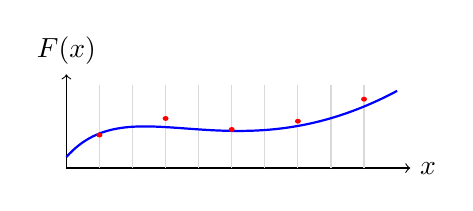
\begin{tikzpicture}[x=0.42cm,y=0.35cm]
 \draw[->] (0,0)--(10.4,0) node[right] {$x$};
 \draw[->] (0,0)--(0,3.4) node[above] {$F(x)$};
 \foreach \x in {1,...,9} {\draw[gray!30] (\x,0)--(\x,3);}
 \draw[blue,thick] (0,0.4) .. controls (2,3.1) and (5,-0.4) .. (10,2.8);
 \foreach \x/\y in {1/1.2,3/1.8,5/1.4,7/1.7,9/2.5}
   \fill[red] (\x,\y) circle (0.09);
\end{tikzpicture}
\end{center}
The next comparison uses Theorem~\ref{thm:32} and Equation~\ref{eq:33}. The proof separates the algebraic estimate from the geometric example. This makes the document useful for edits to prose, formulas, headings and diagrams, while retaining enough ordinary text to exercise paragraph breaking and natural pagination.

\lipsum[18]

\section{A changing estimate: case 035}\label{unit:34}
An observer can return to an earlier part of the document while compilation continues. The relevant statement, equation and hyperlink must still belong to the page actually displayed, including when line wrapping pushes a later theorem across a page boundary.

\lipsum[13-14]
\begin{align}\label{eq:34}
 F_k(x+h)&=F_k(x)+hF_k'(x)+\frac{h^2}{2}F_k''(x)+O(h^3),\\
 \int_0^1 t^k(1-t)\,dt&=\frac{1}{(k+1)(k+2)}.
\end{align}
\begin{theorem}\label{thm:34}
For the finite family in case 35, the normalized error is bounded by $C_k h^2$ whenever $0<h<1$. The constant may depend on $k$ but is independent of the location of the edited paragraph.
\end{theorem}
\begin{proof}
Expand the two terms, collect their first-order contributions, and apply the
triangle inequality. The remaining integral is bounded on the compact interval,
so the asserted estimate follows. This argument also applies after a line break
moves the statement to the next page.
\end{proof}
The next comparison uses Theorem~\ref{thm:33} and Equation~\ref{eq:34}. A local change should remain attached to its source even when surrounding material moves. We compare the displayed argument with the current source version, rather than treating the last compiled page number as a permanent identity.

\lipsum[23]

\section{A changing estimate: case 036}\label{unit:35}
The proof separates the algebraic estimate from the geometric example. This makes the document useful for edits to prose, formulas, headings and diagrams, while retaining enough ordinary text to exercise paragraph breaking and natural pagination.

\lipsum[16-17]
\begin{align}\label{eq:35}
 F_k(x+h)&=F_k(x)+hF_k'(x)+\frac{h^2}{2}F_k''(x)+O(h^3),\\
 \int_0^1 t^k(1-t)\,dt&=\frac{1}{(k+1)(k+2)}.
\end{align}
\begin{theorem}\label{thm:35}
For the finite family in case 36, the normalized error is bounded by $C_k h^2$ whenever $0<h<1$. The constant may depend on $k$ but is independent of the location of the edited paragraph.
\end{theorem}
\begin{proof}
Expand the two terms, collect their first-order contributions, and apply the
triangle inequality. The remaining integral is bounded on the compact interval,
so the asserted estimate follows. This argument also applies after a line break
moves the statement to the next page.
\end{proof}
The next comparison uses Theorem~\ref{thm:34} and Equation~\ref{eq:35}. The construction uses a finite family of examples with different paragraph lengths. Some sentences are short. Others follow the dependence of an estimate on its parameters, introduce a counterexample, and explain why a nearby bound must be reconsidered after an insertion.

\lipsum[3]

\section{A changing estimate: case 037}\label{unit:36}
A local change should remain attached to its source even when surrounding material moves. We compare the displayed argument with the current source version, rather than treating the last compiled page number as a permanent identity.

\lipsum[19-20]
\begin{align}\label{eq:36}
 F_k(x+h)&=F_k(x)+hF_k'(x)+\frac{h^2}{2}F_k''(x)+O(h^3),\\
 \int_0^1 t^k(1-t)\,dt&=\frac{1}{(k+1)(k+2)}.
\end{align}
\begin{lemma}\label{thm:36}
For the finite family in case 37, the normalized error is bounded by $C_k h^2$ whenever $0<h<1$. The constant may depend on $k$ but is independent of the location of the edited paragraph.
\end{lemma}
\begin{proof}
Expand the two terms, collect their first-order contributions, and apply the
triangle inequality. The remaining integral is bounded on the compact interval,
so the asserted estimate follows. This argument also applies after a line break
moves the statement to the next page.
\end{proof}
The next comparison uses Theorem~\ref{thm:35} and Equation~\ref{eq:36}. An observer can return to an earlier part of the document while compilation continues. The relevant statement, equation and hyperlink must still belong to the page actually displayed, including when line wrapping pushes a later theorem across a page boundary.

\lipsum[8]

\section{A changing estimate: case 038}\label{unit:37}
The construction uses a finite family of examples with different paragraph lengths. Some sentences are short. Others follow the dependence of an estimate on its parameters, introduce a counterexample, and explain why a nearby bound must be reconsidered after an insertion.

\lipsum[22-23]
\begin{align}\label{eq:37}
 F_k(x+h)&=F_k(x)+hF_k'(x)+\frac{h^2}{2}F_k''(x)+O(h^3),\\
 \int_0^1 t^k(1-t)\,dt&=\frac{1}{(k+1)(k+2)}.
\end{align}
\begin{theorem}\label{thm:37}
For the finite family in case 38, the normalized error is bounded by $C_k h^2$ whenever $0<h<1$. The constant may depend on $k$ but is independent of the location of the edited paragraph.
\end{theorem}
\begin{proof}
Expand the two terms, collect their first-order contributions, and apply the
triangle inequality. The remaining integral is bounded on the compact interval,
so the asserted estimate follows. This argument also applies after a line break
moves the statement to the next page.
\end{proof}
The next comparison uses Theorem~\ref{thm:36} and Equation~\ref{eq:37}. The proof separates the algebraic estimate from the geometric example. This makes the document useful for edits to prose, formulas, headings and diagrams, while retaining enough ordinary text to exercise paragraph breaking and natural pagination.

\lipsum[13]

\section{A changing estimate: case 039}\label{unit:38}
An observer can return to an earlier part of the document while compilation continues. The relevant statement, equation and hyperlink must still belong to the page actually displayed, including when line wrapping pushes a later theorem across a page boundary.

\lipsum[25-26]
\begin{align}\label{eq:38}
 F_k(x+h)&=F_k(x)+hF_k'(x)+\frac{h^2}{2}F_k''(x)+O(h^3),\\
 \int_0^1 t^k(1-t)\,dt&=\frac{1}{(k+1)(k+2)}.
\end{align}
\begin{theorem}\label{thm:38}
For the finite family in case 39, the normalized error is bounded by $C_k h^2$ whenever $0<h<1$. The constant may depend on $k$ but is independent of the location of the edited paragraph.
\end{theorem}
\begin{proof}
Expand the two terms, collect their first-order contributions, and apply the
triangle inequality. The remaining integral is bounded on the compact interval,
so the asserted estimate follows. This argument also applies after a line break
moves the statement to the next page.
\end{proof}
The next comparison uses Theorem~\ref{thm:37} and Equation~\ref{eq:38}. A local change should remain attached to its source even when surrounding material moves. We compare the displayed argument with the current source version, rather than treating the last compiled page number as a permanent identity.

\lipsum[18]

\section{A changing estimate: case 040}\label{unit:39}
The proof separates the algebraic estimate from the geometric example. This makes the document useful for edits to prose, formulas, headings and diagrams, while retaining enough ordinary text to exercise paragraph breaking and natural pagination.

\lipsum[28-29]
\begin{align}\label{eq:39}
 F_k(x+h)&=F_k(x)+hF_k'(x)+\frac{h^2}{2}F_k''(x)+O(h^3),\\
 \int_0^1 t^k(1-t)\,dt&=\frac{1}{(k+1)(k+2)}.
\end{align}
\begin{lemma}\label{thm:39}
For the finite family in case 40, the normalized error is bounded by $C_k h^2$ whenever $0<h<1$. The constant may depend on $k$ but is independent of the location of the edited paragraph.
\end{lemma}
\begin{proof}
Expand the two terms, collect their first-order contributions, and apply the
triangle inequality. The remaining integral is bounded on the compact interval,
so the asserted estimate follows. This argument also applies after a line break
moves the statement to the next page.
\end{proof}
\begin{center}
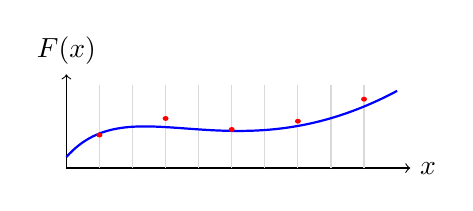
\begin{tikzpicture}[x=0.42cm,y=0.35cm]
 \draw[->] (0,0)--(10.4,0) node[right] {$x$};
 \draw[->] (0,0)--(0,3.4) node[above] {$F(x)$};
 \foreach \x in {1,...,9} {\draw[gray!30] (\x,0)--(\x,3);}
 \draw[blue,thick] (0,0.4) .. controls (2,3.1) and (5,-0.4) .. (10,2.8);
 \foreach \x/\y in {1/1.2,3/1.8,5/1.4,7/1.7,9/2.5}
   \fill[red] (\x,\y) circle (0.09);
\end{tikzpicture}
\end{center}
The next comparison uses Theorem~\ref{thm:38} and Equation~\ref{eq:39}. The construction uses a finite family of examples with different paragraph lengths. Some sentences are short. Others follow the dependence of an estimate on its parameters, introduce a counterexample, and explain why a nearby bound must be reconsidered after an insertion.

\lipsum[23]

\section{A changing estimate: case 041}\label{unit:40}
A local change should remain attached to its source even when surrounding material moves. We compare the displayed argument with the current source version, rather than treating the last compiled page number as a permanent identity.

\lipsum[1-2]
\begin{align}\label{eq:40}
 F_k(x+h)&=F_k(x)+hF_k'(x)+\frac{h^2}{2}F_k''(x)+O(h^3),\\
 \int_0^1 t^k(1-t)\,dt&=\frac{1}{(k+1)(k+2)}.
\end{align}
\begin{theorem}\label{thm:40}
For the finite family in case 41, the normalized error is bounded by $C_k h^2$ whenever $0<h<1$. The constant may depend on $k$ but is independent of the location of the edited paragraph.
\end{theorem}
\begin{proof}
Expand the two terms, collect their first-order contributions, and apply the
triangle inequality. The remaining integral is bounded on the compact interval,
so the asserted estimate follows. This argument also applies after a line break
moves the statement to the next page.
\end{proof}
The next comparison uses Theorem~\ref{thm:39} and Equation~\ref{eq:40}. An observer can return to an earlier part of the document while compilation continues. The relevant statement, equation and hyperlink must still belong to the page actually displayed, including when line wrapping pushes a later theorem across a page boundary.

\lipsum[3]

\section{A changing estimate: case 042}\label{unit:41}
The construction uses a finite family of examples with different paragraph lengths. Some sentences are short. Others follow the dependence of an estimate on its parameters, introduce a counterexample, and explain why a nearby bound must be reconsidered after an insertion.

\lipsum[4-5]
\begin{align}\label{eq:41}
 F_k(x+h)&=F_k(x)+hF_k'(x)+\frac{h^2}{2}F_k''(x)+O(h^3),\\
 \int_0^1 t^k(1-t)\,dt&=\frac{1}{(k+1)(k+2)}.
\end{align}
\begin{theorem}\label{thm:41}
For the finite family in case 42, the normalized error is bounded by $C_k h^2$ whenever $0<h<1$. The constant may depend on $k$ but is independent of the location of the edited paragraph.
\end{theorem}
\begin{proof}
Expand the two terms, collect their first-order contributions, and apply the
triangle inequality. The remaining integral is bounded on the compact interval,
so the asserted estimate follows. This argument also applies after a line break
moves the statement to the next page.
\end{proof}
The next comparison uses Theorem~\ref{thm:40} and Equation~\ref{eq:41}. The proof separates the algebraic estimate from the geometric example. This makes the document useful for edits to prose, formulas, headings and diagrams, while retaining enough ordinary text to exercise paragraph breaking and natural pagination.

\lipsum[8]

\section{A changing estimate: case 043}\label{unit:42}
\hypertarget{varied:late}{}\label{anchor:late}
\noindent \texttt{LATE-0042}: This uniquely marked paragraph remains visible as nearby text, mathematical statements and section boundaries change.
%<VARIED-CURSOR:late>

An observer can return to an earlier part of the document while compilation continues. The relevant statement, equation and hyperlink must still belong to the page actually displayed, including when line wrapping pushes a later theorem across a page boundary.

\lipsum[7-8]
\begin{align}\label{eq:42}
 F_k(x+h)&=F_k(x)+hF_k'(x)+\frac{h^2}{2}F_k''(x)+O(h^3),\\
 \int_0^1 t^k(1-t)\,dt&=\frac{1}{(k+1)(k+2)}.
\end{align}
\begin{lemma}\label{thm:42}
For the finite family in case 43, the normalized error is bounded by $C_k h^2$ whenever $0<h<1$. The constant may depend on $k$ but is independent of the location of the edited paragraph.
\end{lemma}
\begin{proof}
Expand the two terms, collect their first-order contributions, and apply the
triangle inequality. The remaining integral is bounded on the compact interval,
so the asserted estimate follows. This argument also applies after a line break
moves the statement to the next page.
\end{proof}
The next comparison uses Theorem~\ref{thm:41} and Equation~\ref{eq:42}. A local change should remain attached to its source even when surrounding material moves. We compare the displayed argument with the current source version, rather than treating the last compiled page number as a permanent identity.

\lipsum[13]

\section{A changing estimate: case 044}\label{unit:43}
The proof separates the algebraic estimate from the geometric example. This makes the document useful for edits to prose, formulas, headings and diagrams, while retaining enough ordinary text to exercise paragraph breaking and natural pagination.

\lipsum[10-11]
\begin{align}\label{eq:43}
 F_k(x+h)&=F_k(x)+hF_k'(x)+\frac{h^2}{2}F_k''(x)+O(h^3),\\
 \int_0^1 t^k(1-t)\,dt&=\frac{1}{(k+1)(k+2)}.
\end{align}
\begin{theorem}\label{thm:43}
For the finite family in case 44, the normalized error is bounded by $C_k h^2$ whenever $0<h<1$. The constant may depend on $k$ but is independent of the location of the edited paragraph.
\end{theorem}
\begin{proof}
Expand the two terms, collect their first-order contributions, and apply the
triangle inequality. The remaining integral is bounded on the compact interval,
so the asserted estimate follows. This argument also applies after a line break
moves the statement to the next page.
\end{proof}
The next comparison uses Theorem~\ref{thm:42} and Equation~\ref{eq:43}. The construction uses a finite family of examples with different paragraph lengths. Some sentences are short. Others follow the dependence of an estimate on its parameters, introduce a counterexample, and explain why a nearby bound must be reconsidered after an insertion.

\lipsum[18]

\section*{The end of the experiment}
\hyperref[anchor:early]{Return to the early anchor}; \hyperref[anchor:middle]{return to the middle anchor}; \hyperref[anchor:late]{return to the late anchor}.
\end{document}
